%%%%%%%%%%%%%%%%%%%%%%%%%%%%%%%%%%%%%%%%%%%%%%%%%%%%%%%%%%%%%%%%%%%%%%%%%%%%%%%%%%%%%%%%%%%%%%%%%
%
% Document:      DM  product tree
%
%%%%%%%%%%%%%%%%%%%%%%%%%%%%%%%%%%%%%%%%%%%%%%%%%%%%%%%%%%%%%%%%%%%%%%%%%%%%%%
\documentclass{article}
\usepackage{times,layouts}
\usepackage{tikz,hyperref,amsmath}
\usetikzlibrary{positioning,arrows,shapes,decorations.shapes,shapes.arrows}
\usetikzlibrary{backgrounds,calc}
\usepackage[paperwidth=400cm,paperheight=16cm,
left=-2mm,top=3mm,bottom=0mm,right=0mm,
noheadfoot,marginparwidth=0pt,includemp=false,
textwidth=30cm,textheight=50mm]{geometry}
\newcommand\showpage{%
\setlayoutscale{0.5}\setlabelfont{\tiny}\printheadingsfalse\printparametersfalse
\currentpage\pagedesign}
\hypersetup{pdftitle={DM products }, pdfsubject={Diagram illustrating the
products in LSST DM }, pdfauthor={ William O'Mullane}}
\tikzstyle{tbox}=[rectangle,text centered, text width=30mm]
\tikzstyle{wbbox}=[rectangle, rounded corners=3pt, draw=black, top color=blue!50!white, bottom color=white, very thick, minimum height=12mm, inner sep=2pt, text centered, text width=30mm]
\tikzstyle{pbox}=[rectangle, rounded corners=3pt, draw=black, top color=yellow!50!white, bottom color=white, very thick, minimum height=28pt, inner sep=2pt, text centered, text width=35mm]
\tikzstyle{pline}=[-, thick]
\begin{document}
\begin{tikzpicture}[node distance=0mm]
\node (BULKD) [pbox,] {\textbf{Bulk Distrib}
 };
\node (DACPROP) [pbox,right=1mm of BULKD] {\textbf{Proposal Manager}
 };
\node (DACRM) [pbox,right=1mm of DACPROP] {\textbf{Resource Manager}
 };
\node (BUTLER) [pbox,right=15mm of DACRM] {{\tiny \color{black}1.02C.06.02.01} \newline
\textbf{Data Butler Client}
 };
\node (BUTLERpkg) [tbox,below=3mm of BUTLER.north] {{\tiny \color{black} \begin{verbatim} daf_persistence/db/daf_fmt_* \end{verbatim} }  };
\node (DTR) [pbox,right=1mm of BUTLER] {\textbf{Transport/Repl}
 };
\node (SCICATAR) [pbox,right=1mm of DTR] {{\tiny \color{black}.} \newline
\textbf{Science Cat Archive}
 };
\node (SCIIMGAR) [pbox,right=1mm of SCICATAR] {{\tiny \color{black}.} \newline
\textbf{Science Img Archive}
 };
\node (BUILD) [pbox,right=15mm of SCIIMGAR] {{\tiny \color{black}1.02C.10.02.03.01} \newline
\textbf{Build/Unit Test}
 };
\node (BUILDpkg) [tbox,below=3mm of BUILD.north] {{\tiny \color{black} \begin{verbatim} sconsUtils/base/lsstsw/lsst_build \end{verbatim} }  };
\node (COMMS) [pbox,right=1mm of BUILD] {{\tiny \color{black}1.02C.10.02.03.04} \newline
\textbf{Devel Comm Tools}
 };
\node (DOCS) [pbox,right=1mm of COMMS] {{\tiny \color{black}1.02C.10.02.03.03} \newline
\textbf{Doc Infrastructure}
 };
\node (DOCSpkg) [tbox,below=3mm of DOCS.north] {{\tiny \color{black} \begin{verbatim} lsst-texmf/templates/lsstDoxygen \end{verbatim} }  };
\node (DVCS) [pbox,right=1mm of DOCS] {{\tiny \color{black}1.02C.10.02.03.01} \newline
\textbf{SW Version Control}
 };
\node (ISSUE) [pbox,right=1mm of DVCS] {{\tiny \color{black}1.02C.10.02.03.05} \newline
\textbf{Issue Tracking}
 };
\node (PKG) [pbox,right=1mm of ISSUE] {{\tiny \color{black}1.02C.10.02.03.02} \newline
\textbf{Packaging/Distrib}
 };
\node (PKGpkg) [tbox,below=3mm of PKG.north] {{\tiny \color{black} \begin{verbatim} lsst/shebangtron/lsst_dm_stack_demo \end{verbatim} }  };
\node (BPS) [pbox,right=15mm of PKG] {\textbf{Batch Proc}
 };
\node (INFRASYS) [pbox,right=1mm of BPS] {\textbf{Infra Systems}
 };
\node (TXF) [pbox,right=1mm of INFRASYS] {{\tiny \color{black}.} \newline
\textbf{Task Execution}
 };
\node (CI) [pbox,right=15mm of TXF] {{\tiny \color{black}1.02C.10.02.03.01} \newline
\textbf{Contin Integration}
 };
\node (CIpkg) [tbox,below=3mm of CI.north] {{\tiny \color{black} \begin{verbatim} Jenkins \end{verbatim} }  };
\node (PRECURSR) [pbox,right=1mm of CI] {{\tiny \color{black}1.02C.01.01} \newline
\textbf{Precursor Data}
 };
\node (PRECURSRpkg) [tbox,below=3mm of PRECURSR.north] {{\tiny \color{black} \begin{verbatim} obs_*/validation_data_*/testdata_*/afwdata \end{verbatim} }  };
\node (ITARC) [pbox,right=15mm of PRECURSR] {{\tiny \color{black}.} \newline
\textbf{Archive IT}
 };
\node (ITBASE) [pbox,right=1mm of ITARC] {{\tiny \color{black}.} \newline
\textbf{Base IT}
 };
\node (ALRTDSTR) [pbox,right=15mm of ITBASE] {{\tiny \color{black}1.02C.03.03} \newline
\textbf{Alert Distribution}
 };
\node (ALRTFLTR) [pbox,right=1mm of ALRTDSTR] {{\tiny \color{black}1.02C.03.03} \newline
\textbf{Alert Filtering}
 };
\node (L1OFFL) [pbox,right=1mm of ALRTFLTR] {\textbf{L1 Offline Proc}
 };
\node (L1ONL) [pbox,right=1mm of L1OFFL] {{\tiny \color{black}.} \newline
\textbf{L1 OCS Components}
 };
\node (L1SCI) [pbox,right=1mm of L1ONL] {{\tiny \color{black}.} \newline
\textbf{L1 Science Payloads}
 };
\node (L1SRV) [pbox,right=1mm of L1SCI] {{\tiny \color{black}.} \newline
\textbf{Level 1 Services}
 };
\node (L2QC) [pbox,right=15mm of L1SRV] {{\tiny \color{black}1.02C.04.07} \newline
\textbf{L2 Quality Control}
 };
\node (L2QCpkg) [tbox,below=3mm of L2QC.north] {{\tiny \color{black} \begin{verbatim} validate_drp/verify_metrics/ci_hsc \end{verbatim} }  };
\node (L2SCI) [pbox,right=1mm of L2QC] {{\tiny \color{black}.} \newline
\textbf{L2 Science Payloads}
 };
\node (PRODEX) [pbox,right=1mm of L2SCI] {{\tiny \color{black}.} \newline
\textbf{Production Exec}
 };
\node (LSPJL) [pbox,right=15mm of PRODEX] {{\tiny \color{black}.} \newline
\textbf{LSP JupyterLab}
 };
\node (LSPPRTL) [pbox,right=1mm of LSPJL] {{\tiny \color{black}.} \newline
\textbf{LSP Portal}
 };
\node (LSPWEB) [pbox,right=1mm of LSPPRTL] {{\tiny \color{black}.} \newline
\textbf{LSP Web APIs}
 };
\node (NETARCH) [pbox,right=15mm of LSPWEB] {{\tiny \color{black}1.02C.07.08.06} \newline
\textbf{Arc Extl Net}
 };
\node (NETBASE) [pbox,right=1mm of NETARCH] {{\tiny \color{black}1.02C.07.08.03 (moving to 1.02C.08)} \newline
\textbf{Base Network}
 };
\node (NETCHILE) [pbox,right=1mm of NETBASE] {{\tiny \color{black}.} \newline
\textbf{Chilean Nat}
 };
\node (NETINTLUS) [pbox,right=1mm of NETCHILE] {{\tiny \color{black}.} \newline
\textbf{Int/US WANs}
 };
\node (NETLHN) [pbox,right=1mm of NETINTLUS] {{\tiny \color{black}1.02C.08.03} \newline
\textbf{Long-Haul Nets}
 };
\node (APCORR) [pbox,right=15mm of NETLHN] {{\tiny \color{black}1.02C.04.06} \newline
\textbf{Aperture Corr}
 };
\node (ARTFDET) [pbox,right=1mm of APCORR] {{\tiny \color{black}1.02C.03.01} \newline
\textbf{Artifact Detection}
 };
\node (ARTFDETpkg) [tbox,below=3mm of ARTFDET.north] {{\tiny \color{black} \begin{verbatim} meas_algorithms \end{verbatim} }  };
\node (ARTFINTP) [pbox,right=1mm of ARTFDET] {{\tiny \color{black}1.02C.03.01} \newline
\textbf{Artifact Interp}
 };
\node (ASSOC) [pbox,right=1mm of ARTFINTP] {{\tiny \color{black}1.02C.04.06} \newline
\textbf{Association/Match}
 };
\node (ASTROM) [pbox,right=1mm of ASSOC] {{\tiny \color{black}1.02C.03.07} \newline
\textbf{Astrometric Fit}
 };
\node (ASTROMpkg) [tbox,below=3mm of ASTROM.north] {{\tiny \color{black} \begin{verbatim} jointcal/meas_astrom/meas_mosaic \end{verbatim} }  };
\node (BKGDEST) [pbox,right=1mm of ASTROM] {{\tiny \color{black}1.02C.04.03} \newline
\textbf{Background Estim}
 };
\node (BKGDESTpkg) [tbox,below=3mm of BKGDEST.north] {{\tiny \color{black} \begin{verbatim} meas_algorithms \end{verbatim} }  };
\node (BKGDREF) [pbox,right=1mm of BKGDEST] {{\tiny \color{black}1.02C.04.03} \newline
\textbf{Background Ref}
 };
\node (DASSOC) [pbox,right=1mm of BKGDREF] {{\tiny \color{black}1.02C.03.02} \newline
\textbf{DIAObj Association}
 };
\node (DCRTMPL) [pbox,right=1mm of DASSOC] {{\tiny \color{black}1.02C.03.04} \newline
\textbf{DCR Template Gen}
 };
\node (DEBLEND) [pbox,right=1mm of DCRTMPL] {{\tiny \color{black}1.02C.04.05} \newline
\textbf{Deblending}
 };
\node (DEBLENDpkg) [tbox,below=3mm of DEBLEND.north] {{\tiny \color{black} \begin{verbatim} meas_deblender \end{verbatim} }  };
\node (DECORR) [pbox,right=1mm of DEBLEND] {{\tiny \color{black}1.02C.03.04} \newline
\textbf{Img Decorrelation}
 };
\node (DECORRpkg) [tbox,below=3mm of DECORR.north] {{\tiny \color{black} \begin{verbatim} ip_diffim \end{verbatim} }  };
\node (IMCOADD) [pbox,right=1mm of DECORR] {{\tiny \color{black}1.02C.04.04} \newline
\textbf{Image Coaddition}
 };
\node (IMCOADDpkg) [tbox,below=3mm of IMCOADD.north] {{\tiny \color{black} \begin{verbatim} coadd_utils/coadd_chisquared \end{verbatim} }  };
\node (ISR) [pbox,right=1mm of IMCOADD] {{\tiny \color{black}1.02C.03.01} \newline
\textbf{ISR}
 };
\node (ISRpkg) [tbox,below=3mm of ISR.north] {{\tiny \color{black} \begin{verbatim} pipe_tasks/ip_isr \end{verbatim} }  };
\node (MEASURE) [pbox,right=1mm of ISR] {{\tiny \color{black}1.02C.04.06} \newline
\textbf{Measurement}
 };
\node (MEASUREpkg) [tbox,below=3mm of MEASURE.north] {{\tiny \color{black} \begin{verbatim} meas_base/meas_algorithms/meas_extensions_*/meas_modelfit \end{verbatim} }  };
\node (ORBEP) [pbox,right=1mm of MEASURE] {{\tiny \color{black}.} \newline
\textbf{Orbit/Ephemeris}
 };
\node (PHOTOM) [pbox,right=1mm of ORBEP] {{\tiny \color{black}1.02C.03.07} \newline
\textbf{Photometric Fit}
 };
\node (PHOTOMpkg) [tbox,below=3mm of PHOTOM.north] {{\tiny \color{black} \begin{verbatim} jointcal/meas_mosaic \end{verbatim} }  };
\node (PRPRMOT) [pbox,right=1mm of PHOTOM] {{\tiny \color{black}1.02C.03.05} \newline
\textbf{Proper Motion}
 };
\node (PSFESTLG) [pbox,right=1mm of PRPRMOT] {{\tiny \color{black}1.02C.04.03} \newline
\textbf{PSF Estim Large}
 };
\node (PSFESTSM) [pbox,right=1mm of PSFESTLG] {{\tiny \color{black}1.02C.03.01} \newline
\textbf{PSF Estim Small}
 };
\node (PSFESTSMpkg) [tbox,below=3mm of PSFESTSM.north] {{\tiny \color{black} \begin{verbatim} meas_algorithms \end{verbatim} }  };
\node (PSFMATCH) [pbox,right=1mm of PSFESTSM] {{\tiny \color{black}1.02C.04.04} \newline
\textbf{PSF Matching}
 };
\node (RAWCAL) [pbox,right=1mm of PSFMATCH] {\textbf{Raw Meas Cal}
 };
\node (REFCAT) [pbox,right=1mm of RAWCAL] {{\tiny \color{black}1.02C.03.01} \newline
\textbf{Reference Catalogs}
 };
\node (REFCATpkg) [tbox,below=3mm of REFCAT.north] {{\tiny \color{black} \begin{verbatim} meas_algorithms \end{verbatim} }  };
\node (REFMATCH) [pbox,right=1mm of REFCAT] {{\tiny \color{black}1.02C.03.02} \newline
\textbf{Reference Match}
 };
\node (SPATMOD) [pbox,right=1mm of REFMATCH] {{\tiny \color{black}1.02C.03.01} \newline
\textbf{Spatial Models}
 };
\node (SPATMODpkg) [tbox,below=3mm of SPATMOD.north] {{\tiny \color{black} \begin{verbatim} afw \end{verbatim} }  };
\node (SRCDET) [pbox,right=1mm of SPATMOD] {{\tiny \color{black}1.02C.04.05} \newline
\textbf{Source Detection}
 };
\node (STARGAL) [pbox,right=1mm of SRCDET] {{\tiny \color{black}1.02C.04.06} \newline
\textbf{Star/Galaxy Sep}
 };
\node (TEMPLATE) [pbox,right=1mm of STARGAL] {{\tiny \color{black}1.02C.03.04} \newline
\textbf{Template Storage}
 };
\node (VRBLTY) [pbox,right=1mm of TEMPLATE] {{\tiny \color{black}1.02C.03.04} \newline
\textbf{Variability Char}
 };
\node (CAMDESC) [pbox,right=15mm of VRBLTY] {{\tiny \color{black}1.02C.03.05} \newline
\textbf{Camera Descr}
 };
\node (CAMDESCpkg) [tbox,below=3mm of CAMDESC.north] {{\tiny \color{black} \begin{verbatim} afw \end{verbatim} }  };
\node (CHROM) [pbox,right=1mm of CAMDESC] {{\tiny \color{black}1.02C.03.05} \newline
\textbf{Chromaticity Utils}
 };
\node (CHROMpkg) [tbox,below=3mm of CHROM.north] {{\tiny \color{black} \begin{verbatim} afw \end{verbatim} }  };
\node (CONVOL) [pbox,right=1mm of CHROM] {{\tiny \color{black}1.02C.04.01} \newline
\textbf{Convolution}
 };
\node (CONVOLpkg) [tbox,below=3mm of CONVOL.north] {{\tiny \color{black} \begin{verbatim} afw \end{verbatim} }  };
\node (FIELDS) [pbox,right=1mm of CONVOL] {{\tiny \color{black}1.02C.03.05} \newline
\textbf{Approx 2-D Fields}
 };
\node (FIELDSpkg) [tbox,below=3mm of FIELDS.north] {{\tiny \color{black} \begin{verbatim} afw \end{verbatim} }  };
\node (FOOTPRNT) [pbox,right=1mm of FIELDS] {{\tiny \color{black}1.02C.04.01} \newline
\textbf{Footprints}
 };
\node (FOOTPRNTpkg) [tbox,below=3mm of FOOTPRNT.north] {{\tiny \color{black} \begin{verbatim} afw \end{verbatim} }  };
\node (FT) [pbox,right=1mm of FOOTPRNT] {{\tiny \color{black}1.02C.03.05} \newline
\textbf{Fourier Transforms}
 };
\node (FTpkg) [tbox,below=3mm of FT.north] {{\tiny \color{black} \begin{verbatim} afw \end{verbatim} }  };
\node (FUNCTION) [pbox,right=1mm of FT] {{\tiny \color{black}1.02C.03.05} \newline
\textbf{Common Functions}
 };
\node (FUNCTIONpkg) [tbox,below=3mm of FUNCTION.north] {{\tiny \color{black} \begin{verbatim} afw \end{verbatim} }  };
\node (GEOM) [pbox,right=1mm of FUNCTION] {{\tiny \color{black}.} \newline
\textbf{Geometry}
 };
\node (IMAGE) [pbox,right=1mm of GEOM] {{\tiny \color{black}1.02C.04.01} \newline
\textbf{Images}
 };
\node (IMAGEpkg) [tbox,below=3mm of IMAGE.north] {{\tiny \color{black} \begin{verbatim} afw \end{verbatim} }  };
\node (MCSAMP) [pbox,right=1mm of IMAGE] {{\tiny \color{black}1.02C.04.01} \newline
\textbf{MC Sampling}
 };
\node (MCSAMPpkg) [tbox,below=3mm of MCSAMP.north] {{\tiny \color{black} \begin{verbatim} afw \end{verbatim} }  };
\node (NUMINTEG) [pbox,right=1mm of MCSAMP] {{\tiny \color{black}1.02C.04.01} \newline
\textbf{Num Integration}
 };
\node (NUMINTEGpkg) [tbox,below=3mm of NUMINTEG.north] {{\tiny \color{black} \begin{verbatim} afw \end{verbatim} }  };
\node (NUMOPTIM) [pbox,right=1mm of NUMINTEG] {{\tiny \color{black}1.02C.04.01} \newline
\textbf{Num Optimization}
 };
\node (NUMOPTIMpkg) [tbox,below=3mm of NUMOPTIM.north] {{\tiny \color{black} \begin{verbatim} afw \end{verbatim} }  };
\node (PHOTPRIM) [pbox,right=1mm of NUMOPTIM] {{\tiny \color{black}1.02C.04.01} \newline
\textbf{PhotoCal Repr}
 };
\node (PHOTPRIMpkg) [tbox,below=3mm of PHOTPRIM.north] {{\tiny \color{black} \begin{verbatim} afw \end{verbatim} }  };
\node (PROPSET) [pbox,right=1mm of PHOTPRIM] {{\tiny \color{black}1.02C.06.02.01} \newline
\textbf{Property/Metadata}
 };
\node (PROPSETpkg) [tbox,below=3mm of PROPSET.north] {{\tiny \color{black} \begin{verbatim} daf_base \end{verbatim} }  };
\node (PSF) [pbox,right=1mm of PROPSET] {{\tiny \color{black}1.02C.03.05} \newline
\textbf{Point-Spread Funcs}
 };
\node (PSFpkg) [tbox,below=3mm of PSF.north] {{\tiny \color{black} \begin{verbatim} meas_algorithms/shapelet \end{verbatim} }  };
\node (RANDOM) [pbox,right=1mm of PSF] {{\tiny \color{black}1.02C.04.01} \newline
\textbf{Random Numbers}
 };
\node (RANDOMpkg) [tbox,below=3mm of RANDOM.north] {{\tiny \color{black} \begin{verbatim} afw \end{verbatim} }  };
\node (SCITOOLS) [pbox,right=1mm of RANDOM] {{\tiny \color{black}1.02C.04.01} \newline
\textbf{Science Tools}
 };
\node (SCITOOLSpkg) [tbox,below=3mm of SCITOOLS.north] {{\tiny \color{black} \begin{verbatim} afw/utils \end{verbatim} }  };
\node (STATS) [pbox,right=1mm of SCITOOLS] {{\tiny \color{black}1.02C.04.01} \newline
\textbf{Basic Statistics}
 };
\node (STATSpkg) [tbox,below=3mm of STATS.north] {{\tiny \color{black} \begin{verbatim} afw \end{verbatim} }  };
\node (TABLE) [pbox,right=1mm of STATS] {{\tiny \color{black}1.02C.04.01} \newline
\textbf{Tables}
 };
\node (TABLEpkg) [tbox,below=3mm of TABLE.north] {{\tiny \color{black} \begin{verbatim} afw \end{verbatim} }  };
\node (TREES) [pbox,right=1mm of TABLE] {{\tiny \color{black}1.02C.03.05} \newline
\textbf{Tree Structures}
 };
\node (TREESpkg) [tbox,below=3mm of TREES.north] {{\tiny \color{black} \begin{verbatim} afw \end{verbatim} }  };
\node (WARP) [pbox,right=1mm of TREES] {{\tiny \color{black}1.02C.04.01} \newline
\textbf{Warping}
 };
\node (WARPpkg) [tbox,below=3mm of WARP.north] {{\tiny \color{black} \begin{verbatim} afw \end{verbatim} }  };
\node (SQALERT) [pbox,right=15mm of WARP] {{\tiny \color{black}1.02C.10.02.01.04} \newline
\textbf{Alert QC}
 };
\node (SQHARN) [pbox,right=1mm of SQALERT] {{\tiny \color{black}1.02C.10.02.01.01} \newline
\textbf{QC Harness}
 };
\node (SQHARNpkg) [tbox,below=3mm of SQHARN.north] {{\tiny \color{black} \begin{verbatim} validate_base \end{verbatim} }  };
\node (SQNOTIF) [pbox,right=1mm of SQHARN] {{\tiny \color{black}1.02C.10.02.01.02} \newline
\textbf{QC Notifications}
 };
\node (SQREPORT) [pbox,right=1mm of SQNOTIF] {{\tiny \color{black}1.02C.10.02.01.03} \newline
\textbf{QC Reports}
 };
\node (DAC) [pbox,above=15mm of DACPROP] {{\tiny \color{black}.} \newline
\textbf{Data Access Center}
 };
\node (DBB) [pbox,above=15mm of DTR] {{\tiny \color{black}.} \newline
\textbf{Data Backbone}
 };
\node (DEVEL) [pbox,above=15mm of DOCS] {{\tiny \color{black}.} \newline
\textbf{Developer services}
 };
\node (IDM) [pbox,right=1mm of DEVEL] {\textbf{Identity Manager}
 };
\node (INFRA) [pbox,above=15mm of INFRASYS] {{\tiny \color{black}.} \newline
\textbf{Infrastructure}
 };
\node (INTGTEST) [pbox,above=15mm of PRECURSR] {{\tiny \color{black}.} \newline
\textbf{Integration Test}
 };
\node (ITENV) [pbox,above=15mm of ITBASE] {{\tiny \color{black}.} \newline
\textbf{IT Environments}
 };
\node (L1) [pbox,above=15mm of L1OFFL] {{\tiny \color{black}1.02C.03} \newline
\textbf{Level 1 System}
 };
\node (L2) [pbox,above=15mm of L2SCI] {{\tiny \color{black}.} \newline
\textbf{Level 2 System}
 };
\node (LSP) [pbox,above=15mm of LSPPRTL] {{\tiny \color{black}.} \newline
\textbf{Science Platform}
 };
\node (NETDM) [pbox,above=15mm of NETCHILE] {{\tiny \color{black}.} \newline
\textbf{DM Networks}
 };
\node (SCIALG) [pbox,above=15mm of MEASURE] {{\tiny \color{black}.} \newline
\textbf{Science Algorithms}
 };
\node (SCIPRIM) [pbox,above=15mm of NUMINTEG] {{\tiny \color{black}.} \newline
\textbf{Science Primitives}
 };
\node (SQUASH) [pbox,above=15mm of SQHARN] {{\tiny \color{black}.} \newline
\textbf{QC Dashboard}
 };
 \draw[pline]   (BULKD.north) -- ++(0.0,0.5) -| (DAC.south) ; 
 \draw[pline]   (DACPROP.north) -- ++(0.0,0.5) -| (DAC.south) ; 
 \draw[pline]   (DACRM.north) -- ++(0.0,0.5) -| (DAC.south) ; 
 \draw[pline]   (BUTLER.north) -- ++(0.0,0.5) -| (DBB.south) ; 
 \draw[pline]   (DTR.north) -- ++(0.0,0.5) -| (DBB.south) ; 
 \draw[pline]   (SCICATAR.north) -- ++(0.0,0.5) -| (DBB.south) ; 
 \draw[pline]   (SCIIMGAR.north) -- ++(0.0,0.5) -| (DBB.south) ; 
 \draw[pline]   (BUILD.north) -- ++(0.0,0.5) -| (DEVEL.south) ; 
 \draw[pline]   (COMMS.north) -- ++(0.0,0.5) -| (DEVEL.south) ; 
 \draw[pline]   (DOCS.north) -- ++(0.0,0.5) -| (DEVEL.south) ; 
 \draw[pline]   (DVCS.north) -- ++(0.0,0.5) -| (DEVEL.south) ; 
 \draw[pline]   (ISSUE.north) -- ++(0.0,0.5) -| (DEVEL.south) ; 
 \draw[pline]   (PKG.north) -- ++(0.0,0.5) -| (DEVEL.south) ; 
 \draw[pline]   (BPS.north) -- ++(0.0,0.5) -| (INFRA.south) ; 
 \draw[pline]   (INFRASYS.north) -- ++(0.0,0.5) -| (INFRA.south) ; 
 \draw[pline]   (TXF.north) -- ++(0.0,0.5) -| (INFRA.south) ; 
 \draw[pline]   (CI.north) -- ++(0.0,0.5) -| (INTGTEST.south) ; 
 \draw[pline]   (PRECURSR.north) -- ++(0.0,0.5) -| (INTGTEST.south) ; 
 \draw[pline]   (ITARC.north) -- ++(0.0,0.5) -| (ITENV.south) ; 
 \draw[pline]   (ITBASE.north) -- ++(0.0,0.5) -| (ITENV.south) ; 
 \draw[pline]   (ALRTDSTR.north) -- ++(0.0,0.5) -| (L1.south) ; 
 \draw[pline]   (ALRTFLTR.north) -- ++(0.0,0.5) -| (L1.south) ; 
 \draw[pline]   (L1OFFL.north) -- ++(0.0,0.5) -| (L1.south) ; 
 \draw[pline]   (L1ONL.north) -- ++(0.0,0.5) -| (L1.south) ; 
 \draw[pline]   (L1SCI.north) -- ++(0.0,0.5) -| (L1.south) ; 
 \draw[pline]   (L1SRV.north) -- ++(0.0,0.5) -| (L1.south) ; 
 \draw[pline]   (L2QC.north) -- ++(0.0,0.5) -| (L2.south) ; 
 \draw[pline]   (L2SCI.north) -- ++(0.0,0.5) -| (L2.south) ; 
 \draw[pline]   (PRODEX.north) -- ++(0.0,0.5) -| (L2.south) ; 
 \draw[pline]   (LSPJL.north) -- ++(0.0,0.5) -| (LSP.south) ; 
 \draw[pline]   (LSPPRTL.north) -- ++(0.0,0.5) -| (LSP.south) ; 
 \draw[pline]   (LSPWEB.north) -- ++(0.0,0.5) -| (LSP.south) ; 
 \draw[pline]   (NETARCH.north) -- ++(0.0,0.5) -| (NETDM.south) ; 
 \draw[pline]   (NETBASE.north) -- ++(0.0,0.5) -| (NETDM.south) ; 
 \draw[pline]   (NETCHILE.north) -- ++(0.0,0.5) -| (NETDM.south) ; 
 \draw[pline]   (NETINTLUS.north) -- ++(0.0,0.5) -| (NETDM.south) ; 
 \draw[pline]   (NETLHN.north) -- ++(0.0,0.5) -| (NETDM.south) ; 
 \draw[pline]   (APCORR.north) -- ++(0.0,0.5) -| (SCIALG.south) ; 
 \draw[pline]   (ARTFDET.north) -- ++(0.0,0.5) -| (SCIALG.south) ; 
 \draw[pline]   (ARTFINTP.north) -- ++(0.0,0.5) -| (SCIALG.south) ; 
 \draw[pline]   (ASSOC.north) -- ++(0.0,0.5) -| (SCIALG.south) ; 
 \draw[pline]   (ASTROM.north) -- ++(0.0,0.5) -| (SCIALG.south) ; 
 \draw[pline]   (BKGDEST.north) -- ++(0.0,0.5) -| (SCIALG.south) ; 
 \draw[pline]   (BKGDREF.north) -- ++(0.0,0.5) -| (SCIALG.south) ; 
 \draw[pline]   (DASSOC.north) -- ++(0.0,0.5) -| (SCIALG.south) ; 
 \draw[pline]   (DCRTMPL.north) -- ++(0.0,0.5) -| (SCIALG.south) ; 
 \draw[pline]   (DEBLEND.north) -- ++(0.0,0.5) -| (SCIALG.south) ; 
 \draw[pline]   (DECORR.north) -- ++(0.0,0.5) -| (SCIALG.south) ; 
 \draw[pline]   (IMCOADD.north) -- ++(0.0,0.5) -| (SCIALG.south) ; 
 \draw[pline]   (ISR.north) -- ++(0.0,0.5) -| (SCIALG.south) ; 
 \draw[pline]   (MEASURE.north) -- ++(0.0,0.5) -| (SCIALG.south) ; 
 \draw[pline]   (ORBEP.north) -- ++(0.0,0.5) -| (SCIALG.south) ; 
 \draw[pline]   (PHOTOM.north) -- ++(0.0,0.5) -| (SCIALG.south) ; 
 \draw[pline]   (PRPRMOT.north) -- ++(0.0,0.5) -| (SCIALG.south) ; 
 \draw[pline]   (PSFESTLG.north) -- ++(0.0,0.5) -| (SCIALG.south) ; 
 \draw[pline]   (PSFESTSM.north) -- ++(0.0,0.5) -| (SCIALG.south) ; 
 \draw[pline]   (PSFMATCH.north) -- ++(0.0,0.5) -| (SCIALG.south) ; 
 \draw[pline]   (RAWCAL.north) -- ++(0.0,0.5) -| (SCIALG.south) ; 
 \draw[pline]   (REFCAT.north) -- ++(0.0,0.5) -| (SCIALG.south) ; 
 \draw[pline]   (REFMATCH.north) -- ++(0.0,0.5) -| (SCIALG.south) ; 
 \draw[pline]   (SPATMOD.north) -- ++(0.0,0.5) -| (SCIALG.south) ; 
 \draw[pline]   (SRCDET.north) -- ++(0.0,0.5) -| (SCIALG.south) ; 
 \draw[pline]   (STARGAL.north) -- ++(0.0,0.5) -| (SCIALG.south) ; 
 \draw[pline]   (TEMPLATE.north) -- ++(0.0,0.5) -| (SCIALG.south) ; 
 \draw[pline]   (VRBLTY.north) -- ++(0.0,0.5) -| (SCIALG.south) ; 
 \draw[pline]   (CAMDESC.north) -- ++(0.0,0.5) -| (SCIPRIM.south) ; 
 \draw[pline]   (CHROM.north) -- ++(0.0,0.5) -| (SCIPRIM.south) ; 
 \draw[pline]   (CONVOL.north) -- ++(0.0,0.5) -| (SCIPRIM.south) ; 
 \draw[pline]   (FIELDS.north) -- ++(0.0,0.5) -| (SCIPRIM.south) ; 
 \draw[pline]   (FOOTPRNT.north) -- ++(0.0,0.5) -| (SCIPRIM.south) ; 
 \draw[pline]   (FT.north) -- ++(0.0,0.5) -| (SCIPRIM.south) ; 
 \draw[pline]   (FUNCTION.north) -- ++(0.0,0.5) -| (SCIPRIM.south) ; 
 \draw[pline]   (GEOM.north) -- ++(0.0,0.5) -| (SCIPRIM.south) ; 
 \draw[pline]   (IMAGE.north) -- ++(0.0,0.5) -| (SCIPRIM.south) ; 
 \draw[pline]   (MCSAMP.north) -- ++(0.0,0.5) -| (SCIPRIM.south) ; 
 \draw[pline]   (NUMINTEG.north) -- ++(0.0,0.5) -| (SCIPRIM.south) ; 
 \draw[pline]   (NUMOPTIM.north) -- ++(0.0,0.5) -| (SCIPRIM.south) ; 
 \draw[pline]   (PHOTPRIM.north) -- ++(0.0,0.5) -| (SCIPRIM.south) ; 
 \draw[pline]   (PROPSET.north) -- ++(0.0,0.5) -| (SCIPRIM.south) ; 
 \draw[pline]   (PSF.north) -- ++(0.0,0.5) -| (SCIPRIM.south) ; 
 \draw[pline]   (RANDOM.north) -- ++(0.0,0.5) -| (SCIPRIM.south) ; 
 \draw[pline]   (SCITOOLS.north) -- ++(0.0,0.5) -| (SCIPRIM.south) ; 
 \draw[pline]   (STATS.north) -- ++(0.0,0.5) -| (SCIPRIM.south) ; 
 \draw[pline]   (TABLE.north) -- ++(0.0,0.5) -| (SCIPRIM.south) ; 
 \draw[pline]   (TREES.north) -- ++(0.0,0.5) -| (SCIPRIM.south) ; 
 \draw[pline]   (WARP.north) -- ++(0.0,0.5) -| (SCIPRIM.south) ; 
 \draw[pline]   (SQALERT.north) -- ++(0.0,0.5) -| (SQUASH.south) ; 
 \draw[pline]   (SQHARN.north) -- ++(0.0,0.5) -| (SQUASH.south) ; 
 \draw[pline]   (SQNOTIF.north) -- ++(0.0,0.5) -| (SQUASH.south) ; 
 \draw[pline]   (SQREPORT.north) -- ++(0.0,0.5) -| (SQUASH.south) ; 
\node (DM) [wbbox, above=15mm of ITENV]{\textbf{Data Management}};
 \draw[pline]   (DAC.north) -- ++(0.0,0.5) -| (DM.south) ; 
 \draw[pline]   (DBB.north) -- ++(0.0,0.5) -| (DM.south) ; 
 \draw[pline]   (DEVEL.north) -- ++(0.0,0.5) -| (DM.south) ; 
 \draw[pline]   (IDM.north) -- ++(0.0,0.5) -| (DM.south) ; 
 \draw[pline]   (INFRA.north) -- ++(0.0,0.5) -| (DM.south) ; 
 \draw[pline]   (INTGTEST.north) -- ++(0.0,0.5) -| (DM.south) ; 
 \draw[pline]   (ITENV.north) -- ++(0.0,0.5) -| (DM.south) ; 
 \draw[pline]   (L1.north) -- ++(0.0,0.5) -| (DM.south) ; 
 \draw[pline]   (L2.north) -- ++(0.0,0.5) -| (DM.south) ; 
 \draw[pline]   (LSP.north) -- ++(0.0,0.5) -| (DM.south) ; 
 \draw[pline]   (NETDM.north) -- ++(0.0,0.5) -| (DM.south) ; 
 \draw[pline]   (SCIALG.north) -- ++(0.0,0.5) -| (DM.south) ; 
 \draw[pline]   (SCIPRIM.north) -- ++(0.0,0.5) -| (DM.south) ; 
 \draw[pline]   (SQUASH.north) -- ++(0.0,0.5) -| (DM.south) ; 
\node (QSERV) [pbox,below=15mm of SCICATAR] {{\tiny \color{black}1.02C.06.02.03} \newline
\textbf{Qserv DBMS}
 };
\node (QSERVpkg) [tbox,below=3mm of QSERV.north] {{\tiny \color{black} \begin{verbatim} qserv/partition/scisql \end{verbatim} }  };
\node (SCICATDB) [pbox,right=1mm of QSERV] {{\tiny \color{black}.} \newline
\textbf{Science Cat DBs}
 };
\node (GMDS) [pbox,right=15mm of SCICATDB] {{\tiny \color{black}1.02C.06.02.05} \newline
\textbf{Global Metadata}
 };
\node (PRVDB) [pbox,right=1mm of GMDS] {{\tiny \color{black}1.02C.06.01.01} \newline
\textbf{Provenance DB}
 };
\node (ACTIVATR) [pbox,right=15mm of PRVDB] {{\tiny \color{black}1.02C.06.03} \newline
\textbf{Activator Bases}
 };
\node (CONFIG) [pbox,right=1mm of ACTIVATR] {{\tiny \color{black}1.02C.06.03} \newline
\textbf{Pipeline Config}
 };
\node (CONFIGpkg) [tbox,below=3mm of CONFIG.north] {{\tiny \color{black} \begin{verbatim} pex_config \end{verbatim} }  };
\node (LOG) [pbox,right=1mm of CONFIG] {{\tiny \color{black}1.02C.06.04.01} \newline
\textbf{Logging}
 };
\node (LOGpkg) [tbox,below=3mm of LOG.north] {{\tiny \color{black} \begin{verbatim} log \end{verbatim} }  };
\node (MULTCORE) [pbox,right=1mm of LOG] {{\tiny \color{black}1.02C.06.03} \newline
\textbf{Multi-Core Task}
 };
\node (MULTNODE) [pbox,right=1mm of MULTCORE] {{\tiny \color{black}1.02C.06.03} \newline
\textbf{Multi-Node Task}
 };
\node (MULTNODEpkg) [tbox,below=3mm of MULTNODE.north] {{\tiny \color{black} \begin{verbatim} pipe_base/ctrl_pool \end{verbatim} }  };
\node (SPRTASK) [pbox,right=1mm of MULTNODE] {{\tiny \color{black}1.02C.06.03} \newline
\textbf{SuperTask}
 };
\node (SPRTASKpkg) [tbox,below=3mm of SPRTASK.north] {{\tiny \color{black} \begin{verbatim} pipe_supertask/pipe_base/pex_exceptions \end{verbatim} }  };
\node (CTRENV) [pbox,right=15mm of SPRTASK] {\textbf{Archive Center Env}
 };
\node (DACENV) [pbox,right=1mm of CTRENV] {\textbf{Archive DAC Env}
 };
\node (DACINTGR) [pbox,right=1mm of DACENV] {\textbf{DAC Integ Env}
 };
\node (DBBENV) [pbox,right=1mm of DACINTGR] {\textbf{Archive DBB Env}
 };
\node (DBBINTGR) [pbox,right=1mm of DBBENV] {\textbf{DBB Integ Env}
 };
\node (DEVENV) [pbox,right=1mm of DBBINTGR] {\textbf{Dev Env}
 };
\node (L1INTGR) [pbox,right=1mm of DEVENV] {\textbf{L1 Integration Env}
 };
\node (L2INTGR) [pbox,right=1mm of L1INTGR] {\textbf{L2 Integration Env}
 };
\node (SATENV) [pbox,right=1mm of L2INTGR] {\textbf{Satellite Env}
 };
\node (SVENV) [pbox,right=1mm of SATENV] {\textbf{Science Valid Env}
 };
\node (BCTRENV) [pbox,right=15mm of SVENV] {\textbf{Base Center Env}
 };
\node (BDACENV) [pbox,right=1mm of BCTRENV] {\textbf{Base DAC Env}
 };
\node (BDBBENV) [pbox,right=1mm of BDACENV] {\textbf{Base DBB Env}
 };
\node (COMMENV) [pbox,right=1mm of BDBBENV] {\textbf{Comm Cluster Env}
 };
\node (ARC) [pbox,right=15mm of COMMENV] {\textbf{Archiver}
 };
\node (ARCpkg) [tbox,below=3mm of ARC.north] {{\tiny \color{black} \begin{verbatim} ctrl_iip \end{verbatim} }  };
\node (CARC) [pbox,right=1mm of ARC] {\textbf{Catchup Archiver}
 };
\node (CARCpkg) [tbox,below=3mm of CARC.north] {{\tiny \color{black} \begin{verbatim} ctrl_iip \end{verbatim} }  };
\node (EFDT) [pbox,right=1mm of CARC] {\textbf{EFD Tranform}
 };
\node (HEADER) [pbox,right=1mm of EFDT] {\textbf{Header Generator}
 };
\node (OCSBAT) [pbox,right=1mm of HEADER] {\textbf{OCS Batch Proc}
 };
\node (OCSBATpkg) [tbox,below=3mm of OCSBAT.north] {{\tiny \color{black} \begin{verbatim} ctrl_iip \end{verbatim} }  };
\node (POINTP) [pbox,right=1mm of OCSBAT] {\textbf{Pointing Publisher}
 };
\node (PRMPT) [pbox,right=1mm of POINTP] {\textbf{Prompt Proc}
 };
\node (PRMPTpkg) [tbox,below=3mm of PRMPT.north] {{\tiny \color{black} \begin{verbatim} ctrl_iip \end{verbatim} }  };
\node (TMG) [pbox,right=1mm of PRMPT] {\textbf{Telem Gateway}
 };
\node (TMGpkg) [tbox,below=3mm of TMG.north] {{\tiny \color{black} \begin{verbatim} ctrl_iip \end{verbatim} }  };
\node (APOFFL) [pbox,right=15mm of TMG] {{\tiny \color{black}.} \newline
\textbf{Offline Alert Prod}
 };
\node (APPRMPT) [pbox,right=1mm of APOFFL] {{\tiny \color{black}.} \newline
\textbf{Prompt Alert Prod}
 };
\node (AUXTEL) [pbox,right=1mm of APPRMPT] {{\tiny \color{black}1.02C.04.02} \newline
\textbf{Aux Tel Spec Pipe}
 };
\node (CALDAILY) [pbox,right=1mm of AUXTEL] {{\tiny \color{black}1.02C.04.02} \newline
\textbf{Daily Calibration}
 };
\node (CALOFFL) [pbox,right=1mm of CALDAILY] {{\tiny \color{black}1.02C.04.02} \newline
\textbf{Offline Calibration}
 };
\node (CALOFFLpkg) [tbox,below=3mm of CALOFFL.north] {{\tiny \color{black} \begin{verbatim} pipe_drivers \end{verbatim} }  };
\node (CALPRMPT) [pbox,right=1mm of CALOFFL] {{\tiny \color{black}1.02C.04.02} \newline
\textbf{Prompt Calibration}
 };
\node (CALPRMPTpkg) [tbox,below=3mm of CALPRMPT.north] {{\tiny \color{black} \begin{verbatim} pipe_drivers \end{verbatim} }  };
\node (CBPCTRL) [pbox,right=1mm of CALPRMPT] {{\tiny \color{black}1.02C.04.02} \newline
\textbf{CBP Control}
 };
\node (L1QC) [pbox,right=1mm of CBPCTRL] {{\tiny \color{black}1.02C.03} \newline
\textbf{L1 Quality Control}
 };
\node (ARCSRV) [pbox,right=15mm of L1QC] {{\tiny \color{black}.} \newline
\textbf{Archiving Services}
 };
\node (POINTSRV) [pbox,right=1mm of ARCSRV] {\textbf{Pointing Service}
 };
\node (PRMPTSRV) [pbox,right=1mm of POINTSRV] {{\tiny \color{black}.} \newline
\textbf{Prompt Services}
 };
\node (CPPQC) [pbox,right=15mm of PRMPTSRV] {{\tiny \color{black}1.02C.04.02} \newline
\textbf{CPP Quality Control}
 };
\node (CPPSLOW) [pbox,right=1mm of CPPQC] {{\tiny \color{black}1.02C.04.02} \newline
\textbf{Periodic Cal Prod}
 };
\node (CPPYEAR) [pbox,right=1mm of CPPSLOW] {{\tiny \color{black}1.02C.04.02} \newline
\textbf{Annual Cal Prod}
 };
\node (DRP) [pbox,right=1mm of CPPYEAR] {{\tiny \color{black}.} \newline
\textbf{Data Release Prod}
 };
\node (DRPDB) [pbox,right=1mm of DRP] {{\tiny \color{black}1.02C.06.01.01} \newline
\textbf{DRP-Internal DB}
 };
\node (DRPDBpkg) [tbox,below=3mm of DRPDB.north] {{\tiny \color{black} \begin{verbatim} daf_ingest \end{verbatim} }  };
\node (TMPLGEN) [pbox,right=1mm of DRPDB] {{\tiny \color{black}1.02C.03.04} \newline
\textbf{Template Gen Prod}
 };
\node (CMPGN) [pbox,right=15mm of TMPLGEN] {\textbf{Campaign Manager}
 };
\node (JOBACTIV) [pbox,right=1mm of CMPGN] {\textbf{Job Activator}
 };
\node (PREACTIV) [pbox,right=1mm of JOBACTIV] {\textbf{Pre-Flight Activator}
 };
\node (WFM) [pbox,right=1mm of PREACTIV] {\textbf{Workflow Manager}
 };
\node (WFMpkg) [tbox,below=3mm of WFM.north] {{\tiny \color{black} \begin{verbatim} ctrl_orca/ctrl_platform_*/ctrl_execute/ctrl_stats/ctrl_provenance \end{verbatim} }  };
\node (WLM) [pbox,right=1mm of WFM] {\textbf{Workload Manager}
 };
\node (JLACTIV) [pbox,right=15mm of WLM] {{\tiny \color{black}1.02C.10.02.02.05} \newline
\textbf{JupyterLab Activator}
 };
\node (JLDPLY) [pbox,right=1mm of JLACTIV] {{\tiny \color{black}1.02C.10.02.02.06} \newline
\textbf{JupyterLab Deploy}
 };
\node (JLENV) [pbox,right=1mm of JLDPLY] {{\tiny \color{black}1.02C.10.02.02.01} \newline
\textbf{JupyterLab Env}
 };
\node (JLSUIT) [pbox,right=1mm of JLENV] {{\tiny \color{black}1.02C.05.07} \newline
\textbf{JupyterLab SUIT Intf}
 };
\node (JLSW) [pbox,right=1mm of JLSUIT] {{\tiny \color{black}1.02C.10.02.02.04} \newline
\textbf{JupyterLab SW Env}
 };
\node (FFLYAPI) [pbox,right=15mm of JLSW] {{\tiny \color{black}1.02C.05.07} \newline
\textbf{Firefly Python APIs}
 };
\node (FFLYAPIpkg) [tbox,below=3mm of FFLYAPI.north] {{\tiny \color{black} \begin{verbatim} firefly_client \end{verbatim} }  };
\node (FIREFLY) [pbox,right=1mm of FFLYAPI] {{\tiny \color{black}1.02C.05.06 } \newline
\textbf{Firefly}
 };
\node (FIREFLYpkg) [tbox,below=3mm of FIREFLY.north] {{\tiny \color{black} \begin{verbatim} firefly \end{verbatim} }  };
\node (PRTLALRT) [pbox,right=1mm of FIREFLY] {{\tiny \color{black}1.02C.05.09} \newline
\textbf{SUI Alert Interfaces}
 };
\node (PRTLAPPS) [pbox,right=1mm of PRTLALRT] {{\tiny \color{black}1.02C.05.08} \newline
\textbf{Portal Applications}
 };
\node (PRTLINTF) [pbox,right=1mm of PRTLAPPS] {{\tiny \color{black} user workspace} \newline
\textbf{Portal Interfaces}
 };
\node (PRTLINTFpkg) [tbox,below=3mm of PRTLINTF.north] {{\tiny \color{black} \begin{verbatim} Xiuqin Wu \end{verbatim} }  };
\node (PRTLVIS) [pbox,right=1mm of PRTLINTF] {{\tiny \color{black}1.02C.05.07} \newline
\textbf{Visualizers}
 };
\node (DAXCAT) [pbox,right=15mm of PRTLVIS] {{\tiny \color{black}1.02C.06.02.05} \newline
\textbf{Catalog Access}
 };
\node (DAXCATpkg) [tbox,below=3mm of DAXCAT.north] {{\tiny \color{black} \begin{verbatim} dax_dbserv \end{verbatim} }  };
\node (DAXCMETA) [pbox,right=1mm of DAXCAT] {{\tiny \color{black}1.02C.06.02.05} \newline
\textbf{Cat Metadata Acc}
 };
\node (DAXCMETApkg) [tbox,below=3mm of DAXCMETA.north] {{\tiny \color{black} \begin{verbatim} dax_metaserv \end{verbatim} }  };
\node (DAXIMETA) [pbox,right=1mm of DAXCMETA] {{\tiny \color{black}1.02C.06.02.05} \newline
\textbf{Img Metadata Acc}
 };
\node (DAXIMETApkg) [tbox,below=3mm of DAXIMETA.north] {{\tiny \color{black} \begin{verbatim} dax_metaserv \end{verbatim} }  };
\node (DAXIMG) [pbox,right=1mm of DAXIMETA] {{\tiny \color{black}1.02C.06.02.04} \newline
\textbf{Image Access}
 };
\node (DAXIMGpkg) [tbox,below=3mm of DAXIMG.north] {{\tiny \color{black} \begin{verbatim} dax_imgserv \end{verbatim} }  };
\node (DAXWEB) [pbox,right=1mm of DAXIMG] {{\tiny \color{black}1.02C.06.02.02} \newline
\textbf{Web Framework}
 };
\node (DAXWEBpkg) [tbox,below=3mm of DAXWEB.north] {{\tiny \color{black} \begin{verbatim} dax_webserv/dax_webservcommon \end{verbatim} }  };
\node (NETCPAG) [pbox,right=15mm of DAXWEB] {{\tiny \color{black}1.02C.08.03.01.03} \newline
\textbf{Summit - AURA}
 };
\node (NETDWDM) [pbox,right=1mm of NETCPAG] {{\tiny \color{black}1.02C.08.03.01.04} \newline
\textbf{DWDM Equipment}
 };
\node (NETLSAG) [pbox,right=1mm of NETDWDM] {{\tiny \color{black}1.02C.08.03.01.01A} \newline
\textbf{La Serena - AURA}
 };
\node (NETLSSCL) [pbox,right=1mm of NETLSAG] {{\tiny \color{black}1.02C.08.03.01.01} \newline
\textbf{La Ser - Santi }
 };
\node (NET100G) [pbox,right=15mm of NETLSSCL] {{\tiny \color{black}1.02C.08.03.02.01} \newline
\textbf{SCL - MIA 100 Gbps }
 };
\node (NETMGT) [pbox,right=1mm of NET100G] {{\tiny \color{black}1.02C.08.03.02.02} \newline
\textbf{Network Mgmt}
 };
\node (NETSPEC) [pbox,right=1mm of NETMGT] {{\tiny \color{black}1.02C.08.03.02.03} \newline
\textbf{SCL - BR Spectrum }
 };
\node (NETUSW) [pbox,right=1mm of NETSPEC] {{\tiny \color{black}1.02C.08.03.02.01} \newline
\textbf{US National WAN}
 };
\node (ATTRIB) [pbox,right=15mm of NETUSW] {{\tiny \color{black}1.02C.03.06} \newline
\textbf{Attribution/Precov}
 };
\node (ATTRIBpkg) [tbox,below=3mm of ATTRIB.north] {{\tiny \color{black} \begin{verbatim} mops_daymops \end{verbatim} }  };
\node (EPHEM) [pbox,right=1mm of ATTRIB] {{\tiny \color{black}1.02C.03.06} \newline
\textbf{Ephemeris Calc}
 };
\node (EPHEMpkg) [tbox,below=3mm of EPHEM.north] {{\tiny \color{black} \begin{verbatim} mops_night \end{verbatim} }  };
\node (ORBFIT) [pbox,right=1mm of EPHEM] {{\tiny \color{black}1.02C.03.06} \newline
\textbf{Orbit Fitting}
 };
\node (ORBMERGE) [pbox,right=1mm of ORBFIT] {{\tiny \color{black}1.02C.03.06} \newline
\textbf{Orbit Merging}
 };
\node (TRACKLET) [pbox,right=1mm of ORBMERGE] {{\tiny \color{black}1.02C.03.06} \newline
\textbf{Tracklet Gen}
 };
\node (TRACKLETpkg) [tbox,below=3mm of TRACKLET.north] {{\tiny \color{black} \begin{verbatim} mops_daymops \end{verbatim} }  };
\node (CARTGEOM) [pbox,right=15mm of TRACKLET] {{\tiny \color{black}1.02C.03.05} \newline
\textbf{Cartesian Geom}
 };
\node (COORD) [pbox,right=1mm of CARTGEOM] {{\tiny \color{black}1.02C.03.05} \newline
\textbf{Coord Transforms}
 };
\node (COORDpkg) [tbox,below=3mm of COORD.north] {{\tiny \color{black} \begin{verbatim} afw/astshim \end{verbatim} }  };
\node (SPHGEOM) [pbox,right=1mm of COORD] {{\tiny \color{black}1.02C.06.04.03} \newline
\textbf{Spherical Geom}
 };
\node (SPHGEOMpkg) [tbox,below=3mm of SPHGEOM.north] {{\tiny \color{black} \begin{verbatim} sphgeom/skypix/skymap/geom/afw \end{verbatim} }  };
 \draw[pline]   (QSERV.north) -- ++(0.0,0.5) -| (SCICATAR.south) ; 
 \draw[pline]   (SCICATDB.north) -- ++(0.0,0.5) -| (SCICATAR.south) ; 
 \draw[pline]   (GMDS.north) -- ++(0.0,0.5) -| (SCIIMGAR.south) ; 
 \draw[pline]   (PRVDB.north) -- ++(0.0,0.5) -| (SCIIMGAR.south) ; 
 \draw[pline]   (ACTIVATR.north) -- ++(0.0,0.5) -| (TXF.south) ; 
 \draw[pline]   (CONFIG.north) -- ++(0.0,0.5) -| (TXF.south) ; 
 \draw[pline]   (LOG.north) -- ++(0.0,0.5) -| (TXF.south) ; 
 \draw[pline]   (MULTCORE.north) -- ++(0.0,0.5) -| (TXF.south) ; 
 \draw[pline]   (MULTNODE.north) -- ++(0.0,0.5) -| (TXF.south) ; 
 \draw[pline]   (SPRTASK.north) -- ++(0.0,0.5) -| (TXF.south) ; 
 \draw[pline]   (CTRENV.north) -- ++(0.0,0.5) -| (ITARC.south) ; 
 \draw[pline]   (DACENV.north) -- ++(0.0,0.5) -| (ITARC.south) ; 
 \draw[pline]   (DACINTGR.north) -- ++(0.0,0.5) -| (ITARC.south) ; 
 \draw[pline]   (DBBENV.north) -- ++(0.0,0.5) -| (ITARC.south) ; 
 \draw[pline]   (DBBINTGR.north) -- ++(0.0,0.5) -| (ITARC.south) ; 
 \draw[pline]   (DEVENV.north) -- ++(0.0,0.5) -| (ITARC.south) ; 
 \draw[pline]   (L1INTGR.north) -- ++(0.0,0.5) -| (ITARC.south) ; 
 \draw[pline]   (L2INTGR.north) -- ++(0.0,0.5) -| (ITARC.south) ; 
 \draw[pline]   (SATENV.north) -- ++(0.0,0.5) -| (ITARC.south) ; 
 \draw[pline]   (SVENV.north) -- ++(0.0,0.5) -| (ITARC.south) ; 
 \draw[pline]   (BCTRENV.north) -- ++(0.0,0.5) -| (ITBASE.south) ; 
 \draw[pline]   (BDACENV.north) -- ++(0.0,0.5) -| (ITBASE.south) ; 
 \draw[pline]   (BDBBENV.north) -- ++(0.0,0.5) -| (ITBASE.south) ; 
 \draw[pline]   (COMMENV.north) -- ++(0.0,0.5) -| (ITBASE.south) ; 
 \draw[pline]   (ARC.north) -- ++(0.0,0.5) -| (L1ONL.south) ; 
 \draw[pline]   (CARC.north) -- ++(0.0,0.5) -| (L1ONL.south) ; 
 \draw[pline]   (EFDT.north) -- ++(0.0,0.5) -| (L1ONL.south) ; 
 \draw[pline]   (HEADER.north) -- ++(0.0,0.5) -| (L1ONL.south) ; 
 \draw[pline]   (OCSBAT.north) -- ++(0.0,0.5) -| (L1ONL.south) ; 
 \draw[pline]   (POINTP.north) -- ++(0.0,0.5) -| (L1ONL.south) ; 
 \draw[pline]   (PRMPT.north) -- ++(0.0,0.5) -| (L1ONL.south) ; 
 \draw[pline]   (TMG.north) -- ++(0.0,0.5) -| (L1ONL.south) ; 
 \draw[pline]   (APOFFL.north) -- ++(0.0,0.5) -| (L1SCI.south) ; 
 \draw[pline]   (APPRMPT.north) -- ++(0.0,0.5) -| (L1SCI.south) ; 
 \draw[pline]   (AUXTEL.north) -- ++(0.0,0.5) -| (L1SCI.south) ; 
 \draw[pline]   (CALDAILY.north) -- ++(0.0,0.5) -| (L1SCI.south) ; 
 \draw[pline]   (CALOFFL.north) -- ++(0.0,0.5) -| (L1SCI.south) ; 
 \draw[pline]   (CALPRMPT.north) -- ++(0.0,0.5) -| (L1SCI.south) ; 
 \draw[pline]   (CBPCTRL.north) -- ++(0.0,0.5) -| (L1SCI.south) ; 
 \draw[pline]   (L1QC.north) -- ++(0.0,0.5) -| (L1SCI.south) ; 
 \draw[pline]   (ARCSRV.north) -- ++(0.0,0.5) -| (L1SRV.south) ; 
 \draw[pline]   (POINTSRV.north) -- ++(0.0,0.5) -| (L1SRV.south) ; 
 \draw[pline]   (PRMPTSRV.north) -- ++(0.0,0.5) -| (L1SRV.south) ; 
 \draw[pline]   (CPPQC.north) -- ++(0.0,0.5) -| (L2SCI.south) ; 
 \draw[pline]   (CPPSLOW.north) -- ++(0.0,0.5) -| (L2SCI.south) ; 
 \draw[pline]   (CPPYEAR.north) -- ++(0.0,0.5) -| (L2SCI.south) ; 
 \draw[pline]   (DRP.north) -- ++(0.0,0.5) -| (L2SCI.south) ; 
 \draw[pline]   (DRPDB.north) -- ++(0.0,0.5) -| (L2SCI.south) ; 
 \draw[pline]   (TMPLGEN.north) -- ++(0.0,0.5) -| (L2SCI.south) ; 
 \draw[pline]   (CMPGN.north) -- ++(0.0,0.5) -| (PRODEX.south) ; 
 \draw[pline]   (JOBACTIV.north) -- ++(0.0,0.5) -| (PRODEX.south) ; 
 \draw[pline]   (PREACTIV.north) -- ++(0.0,0.5) -| (PRODEX.south) ; 
 \draw[pline]   (WFM.north) -- ++(0.0,0.5) -| (PRODEX.south) ; 
 \draw[pline]   (WLM.north) -- ++(0.0,0.5) -| (PRODEX.south) ; 
 \draw[pline]   (JLACTIV.north) -- ++(0.0,0.5) -| (LSPJL.south) ; 
 \draw[pline]   (JLDPLY.north) -- ++(0.0,0.5) -| (LSPJL.south) ; 
 \draw[pline]   (JLENV.north) -- ++(0.0,0.5) -| (LSPJL.south) ; 
 \draw[pline]   (JLSUIT.north) -- ++(0.0,0.5) -| (LSPJL.south) ; 
 \draw[pline]   (JLSW.north) -- ++(0.0,0.5) -| (LSPJL.south) ; 
 \draw[pline]   (FFLYAPI.north) -- ++(0.0,0.5) -| (LSPPRTL.south) ; 
 \draw[pline]   (FIREFLY.north) -- ++(0.0,0.5) -| (LSPPRTL.south) ; 
 \draw[pline]   (PRTLALRT.north) -- ++(0.0,0.5) -| (LSPPRTL.south) ; 
 \draw[pline]   (PRTLAPPS.north) -- ++(0.0,0.5) -| (LSPPRTL.south) ; 
 \draw[pline]   (PRTLINTF.north) -- ++(0.0,0.5) -| (LSPPRTL.south) ; 
 \draw[pline]   (PRTLVIS.north) -- ++(0.0,0.5) -| (LSPPRTL.south) ; 
 \draw[pline]   (DAXCAT.north) -- ++(0.0,0.5) -| (LSPWEB.south) ; 
 \draw[pline]   (DAXCMETA.north) -- ++(0.0,0.5) -| (LSPWEB.south) ; 
 \draw[pline]   (DAXIMETA.north) -- ++(0.0,0.5) -| (LSPWEB.south) ; 
 \draw[pline]   (DAXIMG.north) -- ++(0.0,0.5) -| (LSPWEB.south) ; 
 \draw[pline]   (DAXWEB.north) -- ++(0.0,0.5) -| (LSPWEB.south) ; 
 \draw[pline]   (NETCPAG.north) -- ++(0.0,0.5) -| (NETCHILE.south) ; 
 \draw[pline]   (NETDWDM.north) -- ++(0.0,0.5) -| (NETCHILE.south) ; 
 \draw[pline]   (NETLSAG.north) -- ++(0.0,0.5) -| (NETCHILE.south) ; 
 \draw[pline]   (NETLSSCL.north) -- ++(0.0,0.5) -| (NETCHILE.south) ; 
 \draw[pline]   (NET100G.north) -- ++(0.0,0.5) -| (NETINTLUS.south) ; 
 \draw[pline]   (NETMGT.north) -- ++(0.0,0.5) -| (NETINTLUS.south) ; 
 \draw[pline]   (NETSPEC.north) -- ++(0.0,0.5) -| (NETINTLUS.south) ; 
 \draw[pline]   (NETUSW.north) -- ++(0.0,0.5) -| (NETINTLUS.south) ; 
 \draw[pline]   (ATTRIB.north) -- ++(0.0,0.5) -| (ORBEP.south) ; 
 \draw[pline]   (EPHEM.north) -- ++(0.0,0.5) -| (ORBEP.south) ; 
 \draw[pline]   (ORBFIT.north) -- ++(0.0,0.5) -| (ORBEP.south) ; 
 \draw[pline]   (ORBMERGE.north) -- ++(0.0,0.5) -| (ORBEP.south) ; 
 \draw[pline]   (TRACKLET.north) -- ++(0.0,0.5) -| (ORBEP.south) ; 
 \draw[pline]   (CARTGEOM.north) -- ++(0.0,0.5) -| (GEOM.south) ; 
 \draw[pline]   (COORD.north) -- ++(0.0,0.5) -| (GEOM.south) ; 
 \draw[pline]   (SPHGEOM.north) -- ++(0.0,0.5) -| (GEOM.south) ; 
\node (ALERTDB) [pbox,below=15mm of SCICATDB] {{\tiny \color{black}1.02C.03.03} \newline
\textbf{Alert DB}
 };
\node (L1DB) [pbox,right=1mm of ALERTDB] {{\tiny \color{black}1.02C.06.01.01} \newline
\textbf{L1 Catalog DB}
 };
\node (L1DBpkg) [tbox,below=3mm of L1DB.north] {{\tiny \color{black} \begin{verbatim} cat \end{verbatim} }  };
\node (L2DB) [pbox,right=1mm of L1DB] {{\tiny \color{black}1.02C.06.01.01} \newline
\textbf{L2 Catalog DB}
 };
\node (L2DBpkg) [tbox,below=3mm of L2DB.north] {{\tiny \color{black} \begin{verbatim} cat \end{verbatim} }  };
\node (ALRTOFFL) [pbox,right=15mm of L2DB] {{\tiny \color{black}1.02C.03.03} \newline
\textbf{Offline Alert Gen}
 };
\node (MOPS) [pbox,right=1mm of ALRTOFFL] {{\tiny \color{black}1.02C.03.06} \newline
\textbf{Moving Object}
 };
\node (MOPSpkg) [tbox,below=3mm of MOPS.north] {{\tiny \color{black} \begin{verbatim} mops_daymops \end{verbatim} }  };
\node (PRECOV) [pbox,right=1mm of MOPS] {{\tiny \color{black}1.02C.03.04} \newline
\textbf{Precovery}
 };
\node (SFPOFFL) [pbox,right=1mm of PRECOV] {{\tiny \color{black}1.02C.03.01} \newline
\textbf{Offline SFP}
 };
\node (ALERTPIPE) [pbox,right=15mm of SFPOFFL] {{\tiny \color{black}1.02C.03.03} \newline
\textbf{Alert Gen Pipe}
 };
\node (SFPPIPE) [pbox,right=1mm of ALERTPIPE] {{\tiny \color{black}1.02C.03.01} \newline
\textbf{Single Frame Pipe}
 };
\node (SFPPIPEpkg) [tbox,below=3mm of SFPPIPE.north] {{\tiny \color{black} \begin{verbatim} pipe_drivers \end{verbatim} }  };
\node (ARCAT) [pbox,right=15mm of SFPPIPE] {\textbf{Aux Tel Archiver}
 };
\node (ARCCOM) [pbox,right=1mm of ARCAT] {\textbf{ComCam Archiver}
 };
\node (ARCLSST) [pbox,right=1mm of ARCCOM] {\textbf{LSSTCam Archiver}
 };
\node (CARCCOM) [pbox,right=1mm of ARCLSST] {\textbf{ComCam Catchup}
 };
\node (CARCLSST) [pbox,right=1mm of CARCCOM] {\textbf{LSSTCam Catchup}
 };
\node (EFDTSRV) [pbox,right=1mm of CARCLSST] {\textbf{EFD Transf Service}
 };
\node (PRMPTCOM) [pbox,right=15mm of EFDTSRV] {\textbf{ComCam Prompt}
 };
\node (PRMPTLSST) [pbox,right=1mm of PRMPTCOM] {\textbf{LSSTCam Prompt}
 };
\node (COADPIPE) [pbox,right=15mm of PRMPTLSST] {{\tiny \color{black}1.02C.04.04} \newline
\textbf{Coadd and Diff}
 };
\node (COADPIPEpkg) [tbox,below=3mm of COADPIPE.north] {{\tiny \color{black} \begin{verbatim} pipe_drivers \end{verbatim} }  };
\node (COADPROC) [pbox,right=1mm of COADPIPE] {{\tiny \color{black}1.02C.04.05} \newline
\textbf{Coadd Processing}
 };
\node (COADPROCpkg) [tbox,below=3mm of COADPROC.north] {{\tiny \color{black} \begin{verbatim} pipe_drivers \end{verbatim} }  };
\node (DRPPOST) [pbox,right=1mm of COADPROC] {{\tiny \color{black}1.02C.04.06} \newline
\textbf{DRP Postprocessing}
 };
\node (IMGCHAR) [pbox,right=1mm of DRPPOST] {{\tiny \color{black}1.02C.04.03} \newline
\textbf{Image Char and Cal}
 };
\node (IMGCHARpkg) [tbox,below=3mm of IMGCHAR.north] {{\tiny \color{black} \begin{verbatim} pipe_drivers \end{verbatim} }  };
\node (MULTIFIT) [pbox,right=1mm of IMGCHAR] {{\tiny \color{black}1.02C.04.06} \newline
\textbf{Object Char}
 };
\node (OVERLAP) [pbox,right=1mm of MULTIFIT] {{\tiny \color{black}1.02C.04.05} \newline
\textbf{Overlap Resolution}
 };
 \draw[pline]   (ALERTDB.north) -- ++(0.0,0.5) -| (SCICATDB.south) ; 
 \draw[pline]   (L1DB.north) -- ++(0.0,0.5) -| (SCICATDB.south) ; 
 \draw[pline]   (L2DB.north) -- ++(0.0,0.5) -| (SCICATDB.south) ; 
 \draw[pline]   (ALRTOFFL.north) -- ++(0.0,0.5) -| (APOFFL.south) ; 
 \draw[pline]   (MOPS.north) -- ++(0.0,0.5) -| (APOFFL.south) ; 
 \draw[pline]   (PRECOV.north) -- ++(0.0,0.5) -| (APOFFL.south) ; 
 \draw[pline]   (SFPOFFL.north) -- ++(0.0,0.5) -| (APOFFL.south) ; 
 \draw[pline]   (ALERTPIPE.north) -- ++(0.0,0.5) -| (APPRMPT.south) ; 
 \draw[pline]   (SFPPIPE.north) -- ++(0.0,0.5) -| (APPRMPT.south) ; 
 \draw[pline]   (ARCAT.north) -- ++(0.0,0.5) -| (ARCSRV.south) ; 
 \draw[pline]   (ARCCOM.north) -- ++(0.0,0.5) -| (ARCSRV.south) ; 
 \draw[pline]   (ARCLSST.north) -- ++(0.0,0.5) -| (ARCSRV.south) ; 
 \draw[pline]   (CARCCOM.north) -- ++(0.0,0.5) -| (ARCSRV.south) ; 
 \draw[pline]   (CARCLSST.north) -- ++(0.0,0.5) -| (ARCSRV.south) ; 
 \draw[pline]   (EFDTSRV.north) -- ++(0.0,0.5) -| (ARCSRV.south) ; 
 \draw[pline]   (PRMPTCOM.north) -- ++(0.0,0.5) -| (PRMPTSRV.south) ; 
 \draw[pline]   (PRMPTLSST.north) -- ++(0.0,0.5) -| (PRMPTSRV.south) ; 
 \draw[pline]   (COADPIPE.north) -- ++(0.0,0.5) -| (DRP.south) ; 
 \draw[pline]   (COADPROC.north) -- ++(0.0,0.5) -| (DRP.south) ; 
 \draw[pline]   (DRPPOST.north) -- ++(0.0,0.5) -| (DRP.south) ; 
 \draw[pline]   (IMGCHAR.north) -- ++(0.0,0.5) -| (DRP.south) ; 
 \draw[pline]   (MULTIFIT.north) -- ++(0.0,0.5) -| (DRP.south) ; 
 \draw[pline]   (OVERLAP.north) -- ++(0.0,0.5) -| (DRP.south) ; 
\end{tikzpicture}
\end{document}
